\documentclass[tikz,border=12pt]{standalone}
\usetikzlibrary{arrows.meta, positioning}

\tikzset{
  nodebox/.style={
    draw,
    rounded corners=3pt,
    fill=white,
    align=left,
    font=\small,
    minimum width=4.7cm,
    text width=4.7cm,
    inner sep=6pt
  },
  widebox/.style={
    draw,
    rounded corners=3pt,
    fill=white,
    align=left,
    font=\small,
    minimum width=5.6cm,
    text width=5.6cm,
    inner sep=6pt
  },
  data/.style={nodebox, fill=purple!6, draw=purple!55},
  impl/.style={nodebox, fill=green!6, draw=green!45!black},
  core/.style={widebox, fill=orange!9, draw=orange!75!black},
  service/.style={nodebox, fill=blue!5, draw=blue!55},
  bundle/.style={widebox, fill=gray!6, draw=gray!60},
  arrow/.style={-{Latex[length=2.4mm]}, thick},
  softarrow/.style={-{Latex[length=2.4mm]}, thick, dashed}
}

\begin{document}
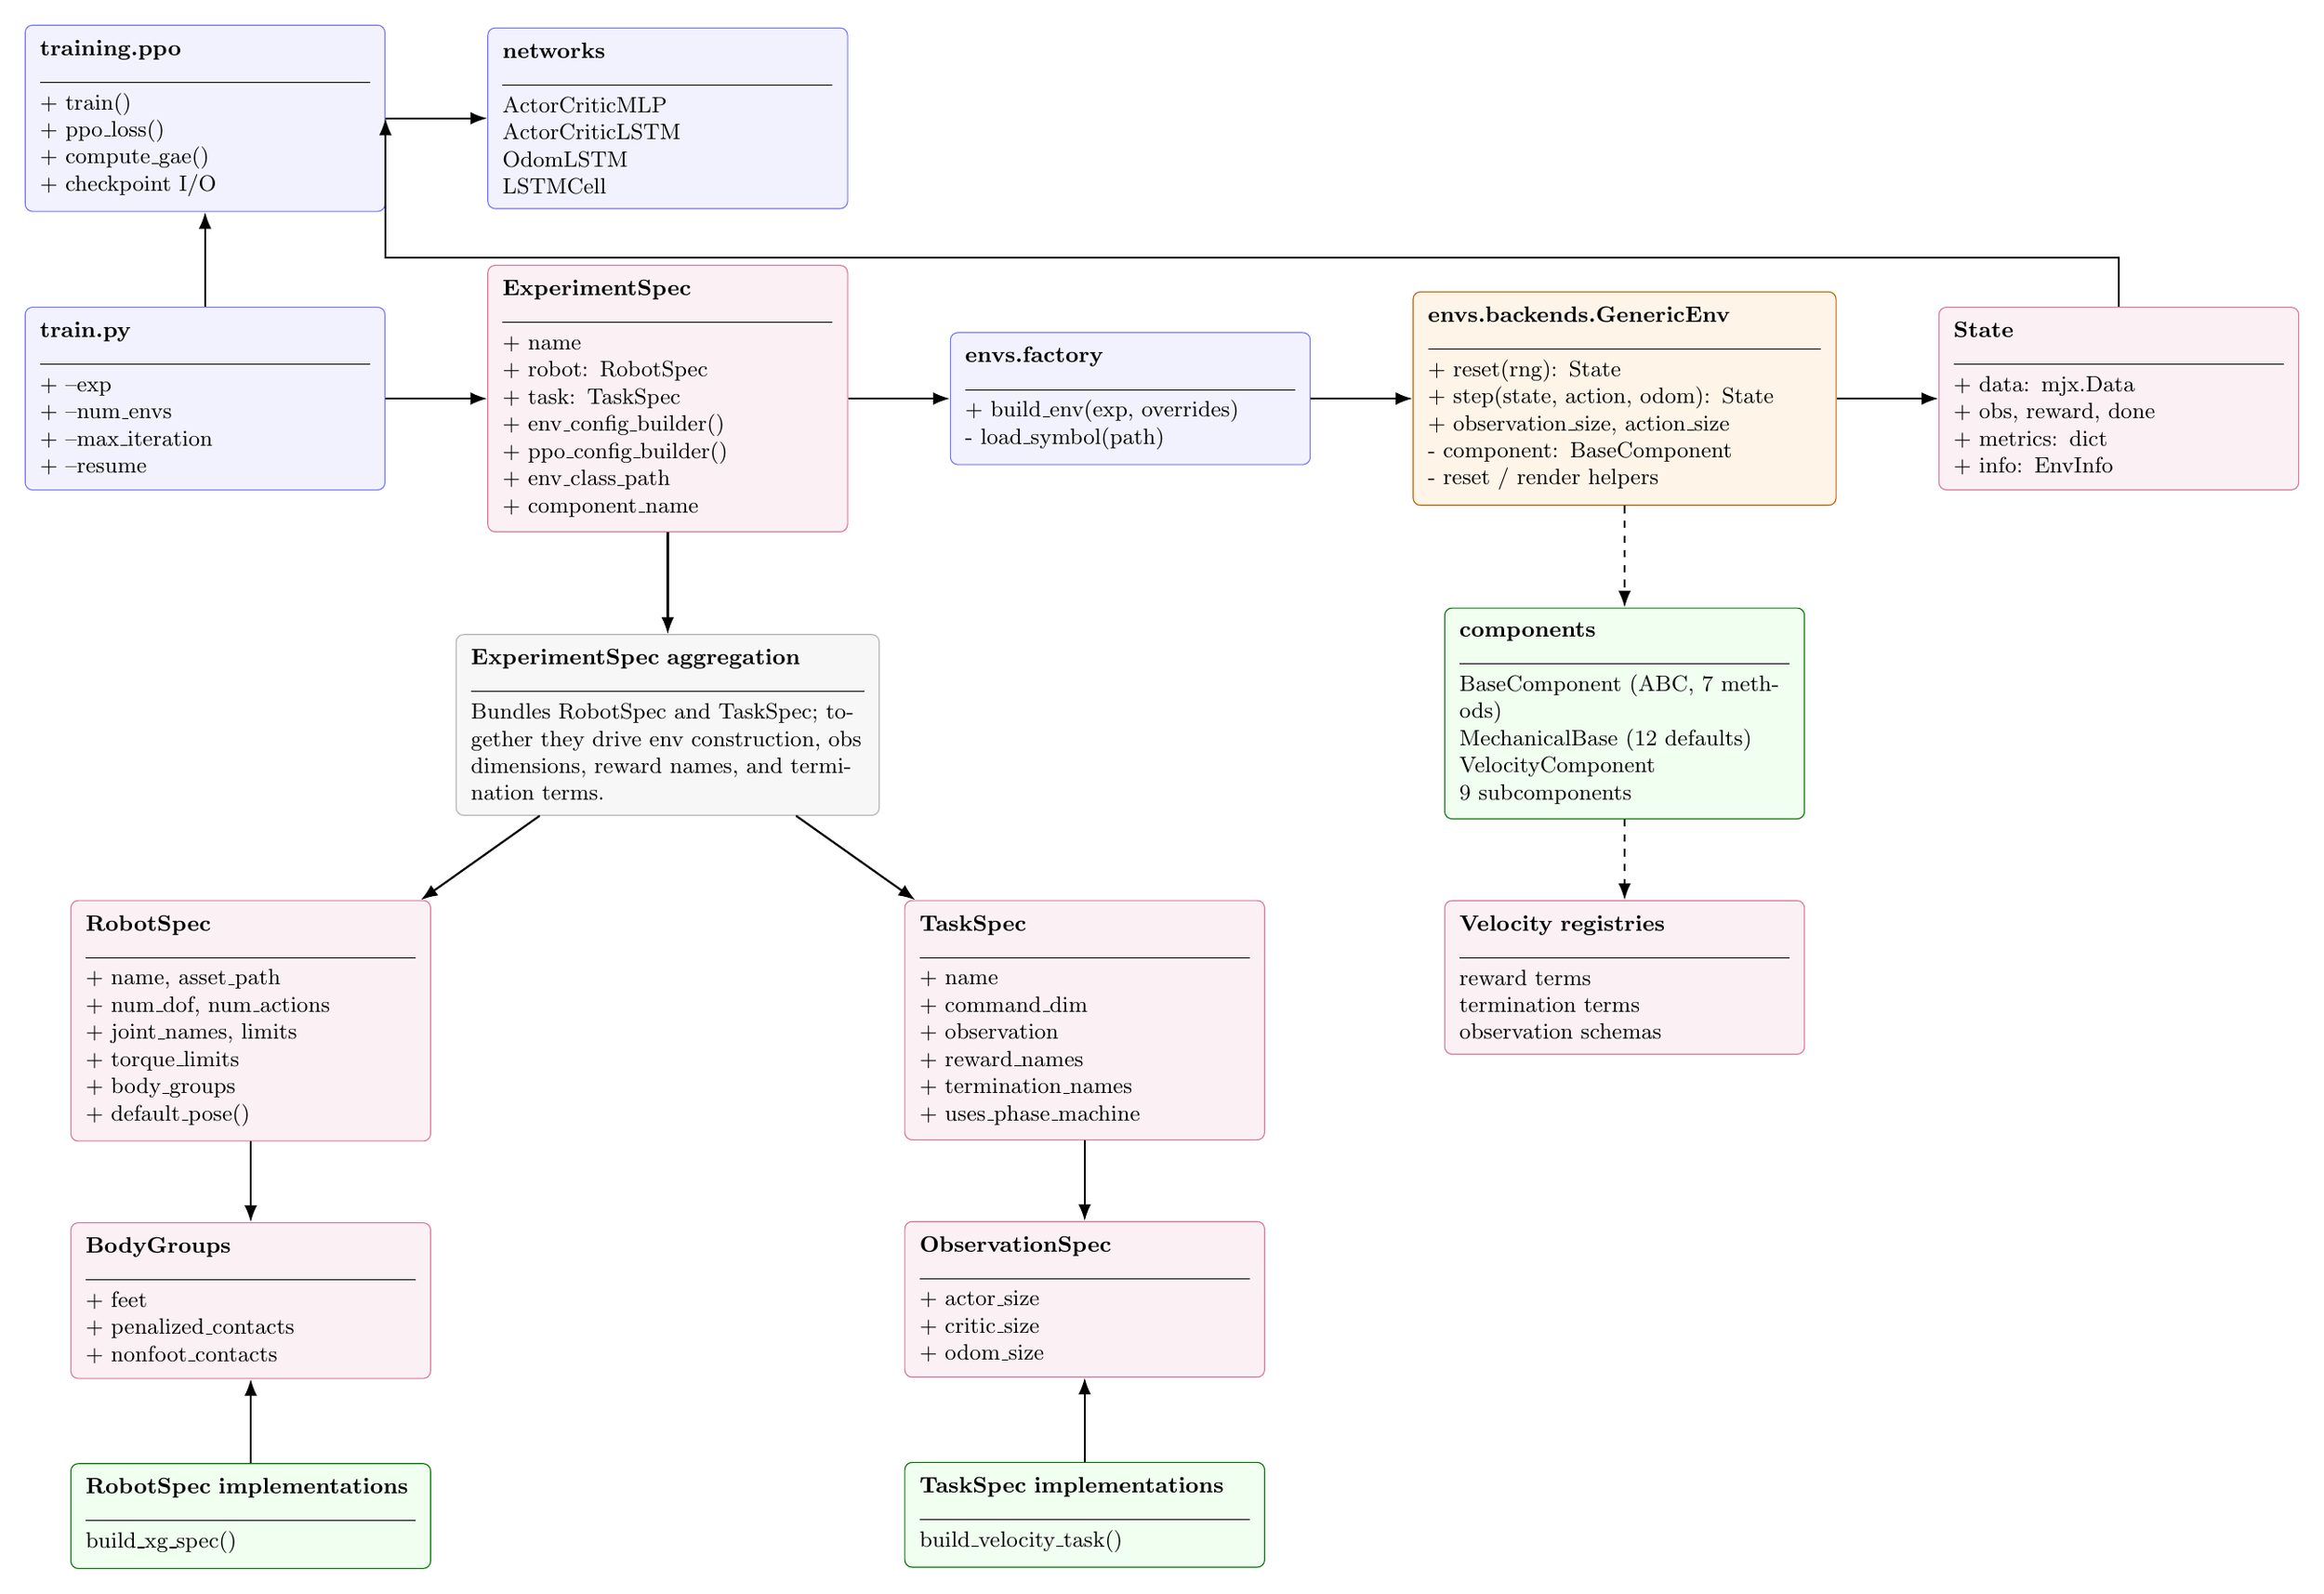
\begin{tikzpicture}[node distance=1.15cm and 1.45cm]

% Main execution chain: one clean horizontal lane.
\node[service] (TrainCLI) {
  \textbf{train.py}\\
  \rule{\linewidth}{0.3pt}\\
  + --exp\\
  + --num\_envs\\
  + --max\_iteration\\
  + --resume
};

\node[data, right=of TrainCLI] (ExperimentSpec) {
  \textbf{ExperimentSpec}\\
  \rule{\linewidth}{0.3pt}\\
  + name\\
  + robot: RobotSpec\\
  + task: TaskSpec\\
  + env\_config\_builder()\\
  + ppo\_config\_builder()\\
  + env\_class\_path\\
  + component\_name
};

\node[service, right=of ExperimentSpec] (EnvFactory) {
  \textbf{envs.factory}\\
  \rule{\linewidth}{0.3pt}\\
  + build\_env(exp, overrides)\\
  - load\_symbol(path)
};

\node[core, right=of EnvFactory] (GenericEnv) {
  \textbf{envs.backends.GenericEnv}\\
  \rule{\linewidth}{0.3pt}\\
  + reset(rng): State\\
  + step(state, action, odom): State\\
  + observation\_size, action\_size\\
  - component: BaseComponent\\
  - reset / render helpers
};

\node[data, right=of GenericEnv] (State) {
  \textbf{State}\\
  \rule{\linewidth}{0.3pt}\\
  + data: mjx.Data\\
  + obs, reward, done\\
  + metrics: dict\\
  + info: EnvInfo
};

% Training lane above the main chain, kept away from specification boxes.
\node[service, above=1.35cm of TrainCLI] (PPO) {
  \textbf{training.ppo}\\
  \rule{\linewidth}{0.3pt}\\
  + train()\\
  + ppo\_loss()\\
  + compute\_gae()\\
  + checkpoint I/O
};

\node[service, right=of PPO] (Networks) {
  \textbf{networks}\\
  \rule{\linewidth}{0.3pt}\\
  ActorCriticMLP\\
  ActorCriticLSTM\\
  OdomLSTM\\
  LSTMCell
};

% Specification lane below ExperimentSpec.
\node[bundle, below=1.45cm of ExperimentSpec] (SpecBundle) {
  \textbf{ExperimentSpec aggregation}\\
  \rule{\linewidth}{0.3pt}\\
  Bundles RobotSpec and TaskSpec; together they drive env construction, obs dimensions, reward names, and termination terms.
};

\node[data, below left=1.2cm and 0.35cm of SpecBundle] (RobotSpec) {
  \textbf{RobotSpec}\\
  \rule{\linewidth}{0.3pt}\\
  + name, asset\_path\\
  + num\_dof, num\_actions\\
  + joint\_names, limits\\
  + torque\_limits\\
  + body\_groups\\
  + default\_pose()
};

\node[data, below right=1.2cm and 0.35cm of SpecBundle] (TaskSpec) {
  \textbf{TaskSpec}\\
  \rule{\linewidth}{0.3pt}\\
  + name\\
  + command\_dim\\
  + observation\\
  + reward\_names\\
  + termination\_names\\
  + uses\_phase\_machine
};

\node[data, below=of RobotSpec] (BodyGroups) {
  \textbf{BodyGroups}\\
  \rule{\linewidth}{0.3pt}\\
  + feet\\
  + penalized\_contacts\\
  + nonfoot\_contacts
};

\node[data, below=of TaskSpec] (ObservationSpec) {
  \textbf{ObservationSpec}\\
  \rule{\linewidth}{0.3pt}\\
  + actor\_size\\
  + critic\_size\\
  + odom\_size
};

% Implementations and components stay in separate vertical lanes.
\node[impl, below=1.2cm of BodyGroups] (RobotImpls) {
  \textbf{RobotSpec implementations}\\
  \rule{\linewidth}{0.3pt}\\
  build\_xg\_spec()
};

\node[impl, below=1.2cm of ObservationSpec] (TaskImpls) {
  \textbf{TaskSpec implementations}\\
  \rule{\linewidth}{0.3pt}\\
  build\_velocity\_task()
};

\node[impl, below=1.45cm of GenericEnv] (Components) {
  \textbf{components}\\
  \rule{\linewidth}{0.3pt}\\
  BaseComponent (ABC, 7 methods)\\
  MechanicalBase (12 defaults)\\
  VelocityComponent\\
  9 subcomponents
};

\node[data, below=of Components] (Schemas) {
  \textbf{Velocity registries}\\
  \rule{\linewidth}{0.3pt}\\
  reward terms\\
  termination terms\\
  observation schemas
};

% Clean arrows: short, local, no long diagonal crossings.
\draw[arrow] (TrainCLI) -- (ExperimentSpec);
\draw[arrow] (ExperimentSpec) -- (EnvFactory);
\draw[arrow] (EnvFactory) -- (GenericEnv);
\draw[arrow] (GenericEnv) -- (State);

\draw[arrow] (TrainCLI.north) -- (PPO.south);
\draw[arrow] (PPO) -- (Networks);
\draw[arrow] (State.north) -- ++(0,0.7) -| (PPO.east);

\draw[arrow] (ExperimentSpec) -- (SpecBundle);
\draw[arrow] (SpecBundle) -- (RobotSpec);
\draw[arrow] (SpecBundle) -- (TaskSpec);
\draw[arrow] (RobotSpec) -- (BodyGroups);
\draw[arrow] (TaskSpec) -- (ObservationSpec);
\draw[arrow] (RobotImpls) -- (BodyGroups);
\draw[arrow] (TaskImpls) -- (ObservationSpec);

\draw[softarrow] (GenericEnv) -- (Components);
\draw[softarrow] (Components) -- (Schemas);

\end{tikzpicture}
\end{document}
